\documentclass[12pt]{article}


\usepackage{graphicx}
\usepackage{colortbl}
\usepackage{xr}
\usepackage{longtable}
\usepackage{xfrac}
\usepackage{tabularx}
\usepackage{booktabs}
\usepackage{hyperref}
\usepackage{xcolor} % for different colour comments
\usepackage{fullpage}
\newcounter{rowcount}
\setcounter{rowcount}{0}


\hypersetup{
    bookmarks=true,         % show bookmarks bar?
      colorlinks=true,       % false: boxed links; true: colored links
    linkcolor=black,          % color of internal links (change box color with linkbordercolor)
    citecolor=green,        % color of links to bibliography
    filecolor=magenta,      % color of file links
    urlcolor=cyan           % color of external links
}

%% Comments
\newif\ifcomments\commentstrue
\ifcomments
\newcommand{\authornote}[3]{\textcolor{#1}{[#3 ---#2]}}
\newcommand{\todo}[1]{\textcolor{red}{[TODO: #1]}}
\else
\newcommand{\authornote}[3]{}
\newcommand{\todo}[1]{}
\fi
\newcommand{\wss}[1]{\authornote{magenta}{SS}{#1}}
\newcommand{\ds}[1]{\authornote{blue}{DS}{#1}}
\newcommand{\kly}[1]{\authornote{green}{KL}{#1}}
\newcommand{\cc}[1]{\authornote{orange}{CC}{#1}}

%%%%%%%%%%%%%%%%%%%%%%%%%%%%%

\begin{document}

\title{Test Report for Quarters} 
\author{Team 6\\ James Anthony (anthonjb)\\ Wenqiang Chen (chenw25)\\ Carolyn Chong 
(chongce)\\ Kevin Ly (lyk2)}
\date{\today}
  
\maketitle

\pagebreak

\tableofcontents
\listoffigures
\listoftables

\section*{Revision History}
\begin{tabular}{|c|c|}
\hline
\textbf{Date}  & \textbf{Comments} \\ \hline
March 20, 2016 & Created first draft. \\ 
\hline
\end{tabular}

\pagebreak

%%%%%%%%%%%%%%%%%%%%%%%%%%%%%

%Introduction
\section{Introduction}
This testing report shows the results of both system tests and non-functional tests on the Quarters application. The system tests are reported based on each individual module. Non-functional tests included tests on usability, performance and robustness.

%Automated Testing
\section{Automated Testing}
\cc{Explain use of automated testing, or explain why it was not feasible for this project.}
All tests that will be automated will be completed for the Final Demo April 1. We will automate testing for every feature, except financing, notification and chat. We will also test the integrity of the database using automated testing. We will also check if every page is reachable, to ensure there are no unhandled HTTP errors. We plan to run automated tests on a weekly basis, every Sunday night. Automated testing tools include Grunt, SinonJS and custom Python scripts. All unit tests will be automated. Since the majority of modules will be Javascript, we will be using QUnit. QUnit is a Javascript unit testing framework. 

%System Tests
\section{System Tests}
\cc{Specific system tests.  All tests should be fully summarized in terms of initial state, input and expected output. Tests should be named. In cases where there are many similar tests just summarize the results. Provide enough info that someone could reproduce your tests. Provide traceability to test plan by referring to test case numbers or modules.} In this section the test cases carried out on each individual module are described. Trivial cases for some modules are not explicitly written out but instead described at a high level. Additional details are provided when necessary.

%4.1 User Registration
\subsection{User Registration} 
\textbf{Test Type:} Functional, Dynamic, Automated. \\
\textbf{Tools Used:} Custom Scripts, Google reCAPTCHA. \\
\textbf{Schedule:} Begin testing November 8. Complete manual tests by PoC Demo November 16. Complete automated dynamic tests by Final Demo April 1. \\
\textbf{Team Member Responsible:} Carolyn Chong.\\
\textbf{Methodology:} The main objective of user registration is to create a user account to be used for login. Users must use a valid email address and pass a user identification procedure. This ensures the user is human and prevents spam and automated scripts from accessing the application and abusing its services. Testing is manual and automated. Manual testing involves people manually going through the registration process in real-time as a user. Automated testing involves systemically attempting SQL injections to test for valid and invalid registrations. Google reCAPTCHA validates that users are legitimate.

\begin{longtable}{|p{2cm}|p{3cm}|p{5cm}|p{5cm}|}
\hline
\textbf{Test Case}  & \textbf{Initial State} & \textbf{Input} & \textbf{Output} \\ \hline
1.1 & Landing page. Empty fields. & Email and password entered and passes reCAPTCHA test. Clicks register. & Verification email sent. Redirected to application main page. \\ 
\hline
1.2 & Landing page. Empty fields. & Empty field(s). Clicks register. & Stays on the same page. Error message appears. Empty field is highlighted. \\
\hline
1.3 & Landing page. Empty fields. & Email address already stored in database. Clicks register. & Stays on the same page. Error message appears. Email field is highlighted. \\
\hline
1.4 & Landing page. Empty fields. & Fails reCAPTCHA test. & Stays on the same page. Error message appears. Test field is highlighted. \\
\hline
\end{longtable}



%4.2 User Login
\subsection{User Login}
\textbf{Test Type:} Functional, Dynamic, Automated. \\
\textbf{Tools Used:} Custom Scripts. \\
\textbf{Schedule:} Begin testing November 8. Complete manual tests by PoC Demo November 16. Complete automated dynamic tests by Final Demo April 1. \\
\textbf{Team Member Responsible:} Carolyn Chong. \\
\textbf{Methodology:} The main objective of user login is to ensure a secure process where only valid users are allowed to enter the application. Testing involves authenticating users against an existing database to determine if they are valid users or not. Testing is automated. Automated testing involves systemically attempting SQL injections to test for valid and invalid logins.

\begin{longtable}{|p{2cm}|p{3cm}|p{5cm}|p{5cm}|}
\hline
\textbf{Test Case}  & \textbf{Initial State} & \textbf{Input} & \textbf{Output} \\ \hline
2.1 & Landing page. Empty username and password fields. & Valid username and password combination. Clicks login. & Redirected to application main page. \\ 
\hline
2.2 & Landing page. Empty username and password fields. & Invalid username and password combination. Clicks login. & Stays on the same page. Error message appears. Fields are highlighted. After 5 unsuccessful attempts, user cannot login for 10 minutes. \\
\hline
2.3 & Landing page. Empty username and password fields. & Empty username and/or password fields. Clicks login. & Stays on the same page. Error message appears. Fields are highlighted. \\
\hline
2.4 & Application main page. & Clicks logout. & User is successfully logged out from system. Redirected to login page. \\
\hline
2.5 & Landing page. Empty username and password fields. User attempting to login on another device while already logged in on a device. & Valid username and password combination. Clicks login. & Stays on the same page. Error message appears. \\ 
\hline
\end{longtable}

%4.3 Calendar
\subsection{Calendar}

\begin{longtable}{|p{1.5cm}|p{1.5cm}|p{1.5cm}|p{2cm}|p{4cm}|p{2cm}|p{1.5cm}|}
\hline
\textbf{No.} & \textbf{Test Case}  & \textbf{Initial State} & \textbf{Input} & \textbf{Expected Output} & \textbf{Actual Output} & \textbf{Result}\\ 
\hline
3.1-3.4 & Add event to Calendar. & Calendar page. & User selects date to add new event, enters information, clicks save. & Modal opens with fields, and closes upon save. Event is updated correctly on Calendar. The same output results if user selects existing event to modify. & As expected. & PASS \\
\hline
3.5 & Delete event from Calendar & Calendar page. & User selects  event to delete, clicks delete. & Modal opens with fields. Upon clicking delete, the modal closes and the event is removed from the Calendar. & As expected. & PASS \\
\hline
\end{longtable}

%4.4 Maintenance Ticketing System
\subsection{Maintenance Tracking}
\textbf{Test Type:} Functional, Dynamic, Static, Automated. \\
\textbf{Tools Used:} QUnit, Chron Scripts. \ds{Chron scripts?}\\
\textbf{Schedule:} Begin testing after the PoC Demo. Complete automated tests by Final Demo April 1. \\
\textbf{Team Member Responsible:} Kevin Ly. \\
\textbf{Methodology:} The maintenance tracking system allows tenants to create maintenance requests, where the landlord then responds and updates with further information. This portion of the system is restricted based on the user type; tenants cannot modify maintenance ticket properties. This component will be tested using unit tests for functionality, with automated testing to ensure the permissions are handled properly. Static database checkers will be used in conjunction with the automated test cases to check for proper database modifications.

\begin{longtable}{|p{2cm}|p{3cm}|p{5cm}|p{5cm}|}
\hline
\textbf{Test Case}  & \textbf{Initial State} & \textbf{Input} & \textbf{Output} \\ \hline
4.1 & Quarters Web Application. & Open maintenance system. & Maintenance system opens and shows new maintenance tickets with existing tickets in chronological order. \\ 
\hline
4.2 & Maintenance System. & Click on maintenance ticket. & Inner dialog opens displaying all properties in a maintenance ticket. \\
\hline
4.3 & Maintenance System. & Entering a search query or adding a filter. & Sort and filter maintenance tickets and reveal only successful tickets. \\
\hline
4.4 & Maintenance Ticket Window. & Modifying properties of a ticket. & Save icon appears in dialog to confirm changes.\\
\hline
4.5 & Maintenance Ticket Window. & Saving ticket properties & Window will close, and database will be updated to reflect changes.\\
\hline
4.6 & Maintenance Ticket Window. & Deleting Ticket. & Confirmation window will appear. Upon deletion confirmation, close window and remove data from database.\\
\hline
4.7 & Maintenance System & Click on create new request. & Opens a new ticket window.\\
\hline
4.8 & New Maintenance ticket window. & Click on create empty fields. & Window will remain opening, prompt will display error message.\\
\hline
4.9 & New Maintenance ticket window. & Click on create, required fields filled. & Window closes, database will be updated with new ticket.\\
\hline
4.10 & New Maintenance ticket window. & Click on cancel with fields filled. & Window remains open, prompt will ask for confirmation on close.\\
\hline
4.11 & Confirmation Prompt. & Click on OK. & Closes prompt and dialog. \\
\hline
4.12 & Confirmation Prompt. & Click on cancel. & Closes prompt, dialog remains open.\\
\hline
\end{longtable}

%4.5 house management
\subsection{House Management}
\textbf{Test Type:} Functional, Dynamic, Automated. \\
\textbf{Tools Used:} QUnit. \\
\textbf{Schedule:} Begin testing after the PoC Demo. Complete automated tests by Final Demo April 1. \\
\textbf{Team Member Responsible:} Kevin Ly.\\
\textbf{Methodology:} The house management system allows users to create, delete, view, and modify information about houses. Unit tests will be created for each function in the feature which will be included in the automated testing sequence.

\begin{longtable}{|p{2cm}|p{3cm}|p{5cm}|p{5cm}|}
\hline
\textbf{Test Case}  & \textbf{Initial State} & \textbf{Input} & \textbf{Output} \\ \hline
5.1 & House Management, not admin. & Click modify information. & Nothing.\\ 
\hline
5.2 & House Management, admin. & Click modify information. & Input fields become editable. \\
\hline
5.3 & House Management, admin. & Modify information fields. & Save button opens, discard changes appears. \\
\hline
5.4 & House Management, any user. & Click on View Documents. & Redirects to new page showing all uploaded documents in House. \\
\hline
5.5 & House Documents, any user. & Clicks on a document. & Retrieves documents and initiates file transfer.\\
\hline
5.6 & House Documents, admin. & Clicks on Add Documents. & Upload window opens for user upload, file will be transfer to server and information is updated in database.\\
\hline
5.7 & House Documents, admin. & Clicks on delete document. & Prompt opens.\\
\hline
5.8 & Deletion prompt, admin. & Clicks on yes. & Prompt closed, file is removed from display, database is updated.\\
\hline
5.9 & Deletion prompt, admin. & Clicks on no. & Prompt closed.\\
\hline
5.10 & House Management, any user. & Clicks on view members. & Shows all memebers of the house and their role.\\
\hline
5.11 & House Management, admin, members list visible. & Clicks on add member. & Dialog will appear.\\
\hline
5.12 & Member Dialog, admin, fields empty. & Clicks on ok. & Prompt opens, notifying missing fields. \\
\hline
5.13 & Member Dialog, admin, fields complete. & Clicks on ok. & Window closes, new user is notified, database is updated, member status pending.\\
\hline
5.14 & Member Dialog, admin. & Clicks on cancel. & Window closes.\\
\hline
\end{longtable}


%4.6 landing page
\subsection{Landing Page}

\begin{longtable}{|p{1.5cm}|p{1.5cm}|p{1.5cm}|p{2cm}|p{4cm}|p{2cm}|p{1.5cm}|}
\hline
\textbf{No.} & \textbf{Test Case}  & \textbf{Initial State} & \textbf{Input} & \textbf{Expected Output} & \textbf{Actual Output} & \textbf{Result}\\ 
\hline
6.1,6.2 & Access login or registration. & Not logged in. & Clicks on login. & Modal opens and email and password fields appear. The same output results if user clicks on register. & As expected. & PASS \\
\hline
\end{longtable}


%4.7 Finance
\subsection{Finance}
\textbf{Test Type:} Functional, Dynamic, Manual. \\
\textbf{Tools Used:} None. \\
\textbf{Schedule:} Begin testing after the PoC Demo. Complete automated tests by Final Demo April 1. \\
\textbf{Team Member Responsible:} James Anthony. \\
\textbf{Methodology:} Tests can be performed by having one user add payment deadlines, and having another user send arbitrary amounts of money via PayPal. Speed and accuracy of transactions can be tracked. Transaction records can be manually evaluated for correctness.

\begin{longtable}{|p{2cm}|p{3cm}|p{5cm}|p{5cm}|}
\hline
\textbf{Test Case} & \textbf{Initial State} & \textbf{Input} & \textbf{Output} \\ \hline
7.1 & No payments due. & User initiates PayPal transaction. & Error message indicating that no payments are due at the current time.\\
\hline
7.2 & No payments due. & User posts payment request with some deadline. & New payment deadline added.\\
\hline
7.3 & Payment due. & User initiates PayPal transaction. & Transaction is handled by PayPal. All users involved are notified of the completed payment. Deadline is removed from list of current payments due.\\
\hline
7.4 & Payment due. & Payment has not been completed, and deadline has passed. & All users involved are notified that the deadline has passed. Deadline is marked as past due, and users will continue to be notified until either the payment has been completed, or the due payment is removed.\\
\hline
7.5 & Payment due. & User who posted the original due payment removes the request. & Payment request is removed from the list of due payments.\\
\hline
\end{longtable}


%4.8 Notification
\subsection{Notifications}
\textbf{Test Type:} Functional, Dynamic, Manual. \\
\textbf{Tools Used:} None. \\
\textbf{Schedule:} Begin testing after the PoC Demo. Complete automated tests by Final Demo April 1. \\
\textbf{Team Member Responsible:} Wenqiang Chen. \\
\textbf{Methodology:} The main objective of notification is to remind user of events that has had happened; users should be notified immediate after the event has taken place. The testing involves one user completing different actions which generates notification and have another user related to this event receive notification.

\begin{longtable}{|p{2cm}|p{3cm}|p{5cm}|p{5cm}|}
\hline
\textbf{Test Case}  & \textbf{Initial State} & \textbf{Input} & \textbf{Output} \\ \hline
8.1 & Main page. User(A) logged in. & User(B) sends money request. & User(A) sees notification of pending payment due.  \\ 
\hline
8.2 & Main page. User(A) logged in. & User(A) pays user(B). & User(B) sees notification of payment completed.  \\ 
\hline
8.3 & Main page. User(A) logged in. & User(A) has late payment. & User(A) sees notification of late payment.  \\ 
\hline
8.4 & Main page. User(A) logged in. & User(A) joins a house.  & Other users in that house sees notification that user(A) joined the house. \\
\hline
8.5 & Main page. User(A)(landlord) logged in. & User(B) sends maintenance ticket(Critical). & User(A) sees notification of unresolved maintenance ticket, receives email, receives text message. \\
\hline
8.6 & Main page. User(A)(landlord) logged in. & User(B) sends maintenance ticket(Major.) & User(A) sees notification of unresolved maintenance ticket, receives email.\\
\hline
8.7 & Main page. User(A)(landlord) logged in. & User(B) sends maintenance ticket(Minor). & User(A) sees notification of unresolved maintenance ticket. \\
\hline
8.8 & Main page. User(A) logged in. & User(B)(Landlord) resolves a maintenance ticket. & User(A) sees notification of resolved maintenance ticket. \\
\hline
8.9 & Main page. User(A) logged in. & User(B) sends user(A) a message. & User(A) sees notification of unread message. \\
\hline
8.10 & Main page. User(A) logged in. & User(B) makes a post in discussion board. & User(A) sees notification of unread post. \\
\hline
8.11 & Main page. User(A) logged in. & User(B) replies to a post made by user(A). & User(A) sees notification of unread reply. \\
\hline
8.12 & Main page. User(A) logged in. & User(A) leaves a house.  & Other users in that house sees notification that user(A) left the house. \\
\hline
8.13 & Main page. User(A) logged in. & User(B) adds event to Calendar. & User(A) sees notification of added post. \\
\hline
8.14 & Main page. User(A) logged in. & User(B) deletes event from Calendar. & User(A) sees notification of deleted event. \\
\hline
8.15 & Main page. User(A) logged in. & User(A)has event happening on day. & User(A) sees notification of event. \\
\hline
8.16 & Main page. User(A) logged in. Notification displayed. & User clicks on Notification icon. & Notification disappears. \\
\hline
\end{longtable}

%4.9 Administrative File Storage
\subsection{Administrative File Storage}
\textbf{Test Type:} Functional, Dynamic, Automated. \\
\textbf{Tools Used:} Custom Scripts. \\
\textbf{Schedule:} Begin testing after the PoC Demo. Complete automated tests by Final Demo April 1. \\
\textbf{Team Member Responsible:} James Anthony. \\
\textbf{Methodology:} A script can be used to test the process of uploading and downloading multiple files of different types and sizes.

\begin{longtable}{|p{2cm}|p{3cm}|p{5cm}|p{5cm}|}
\hline
\textbf{Test Case} & \textbf{Initial State} & \textbf{Input} & \textbf{Output} \\ \hline
9.1 & 0 files in storage. & User tries to upload a file of size $s$, where $s \le$ max file size. & Successful file upload.\\
\hline
9.2 & 0 files in storage. & User tries to upload a file of size $s$, where $s >$ max file size. & Error message indicating file has not been uploaded.\\
\hline
9.3 & $n$ files in storage. & User tries to upload a file of size $s$, where $s \le$ total remaining space. & Successful file upload.\\
\hline
9.4 & $n$ files in storage. & User tries to upload a file of size $s$, where $s >$ total remaining space. & Error message indicating file has not been uploaded.\\
\hline
9.5 & $n$ files in storage. & User tries to upload a file with an invalid type. & Error message indicating file has not been uploaded.\\
\hline
9.6 & $n$ files in storage. & User requests to download a file. & Successful file download.\\
\hline
9.7 & $n$ files in storage. & Connection interrupted while download is in progress. & Error message indicating file has not been downloaded.\\
\hline
9.8 & $n$ files in storage. & User tries to upload  $n > 1$ files. & Error message indicating only one file can be uploaded at a time.\\
\hline
9.9 & $n$ files in storage. & User clicks delete file. & File removed. \\
\hline
\end{longtable}

%4.10 Bulletin Board
\subsection{Bulletin Board}
\textbf{Test Type:} Functional, Dynamic, Automated. \\
\textbf{Tools Used:} Custom Scripts. \\
\textbf{Schedule:} Begin testing after the PoC Demo. Complete automated tests by Final Demo April 1. \\
\textbf{Team Member Responsible:} James Anthony. \\
\textbf{Methodology:} A script can be used to test the process of posting on the discussion board, and commenting on existing posts.

\begin{longtable}{|p{2cm}|p{3cm}|p{5cm}|p{5cm}|}
\hline
\textbf{Test Case} & \textbf{Initial State} & \textbf{Input} & \textbf{Output} \\ \hline
10.1 & No posts on bulletin board. & A post with 0 characters & Empty post is disgarded
\ds{``discarded"}
and not added to bulletin board.\\
\hline
10.2 & No posts on bulletin board. & A post with $n$ characters, where $n > 0$. & Bulletin board is updated with the post of $n$ characters.\\
\hline
10.3 & $p$ posts on bulletin board, where $p > 0$. & A post with 0 characters & Empty post is disgarded and not added to bulletin board.\\
\hline
10.4 & $p$ posts on bulletin board, where $p > 0$. & A post with $n$ characters, where $n > 0$. & Bulletin board is updated with the post of $n$ characters.\\
\hline
10.5 & $p$ posts on bulletin board, where $p > 0$. & A comment with 0 characters on an existing post $p$. & Empty comment is disgarded
\ds{discarded}
and not added to bulletin board.\\
\hline
10.6 & $p$ posts on bulletin board, where $p > 0$. & A comment with $n$ characters where $n > 0$, on an existing post $p_i$. & Comment is added to the list of comments associated with post $p_i$.\\
\hline
\end{longtable}


%5. Non-Functional Tests
\section{Non-Functional Tests}

\subsection{Usability}
The usability of Quarters was evaluated by asking test participants to complete a pre-defined task, as well as a pre- and post-test questionnaire, as outlined in the Test Plan. The participants' performance was measured by the total time to complete the task. The average time of all participants to complete the task on Quarters was measured. ‘Think-aloud’ results provided subjective feedback on the user experience of Quarters. The post-questionnaire provided subjective feedback on Quarters itself.

\subsubsection{Results}
Figure \ref{fig:participants} shows the participants. This data was collected during Task 1. The task completion rate was 100\% for both tasks 2a and 2b, and the average times were both less than 60 seconds. Therefore the success metric stated in the Test Plan was met for completion rate and completion time, as shown in Figure \ref{fig:task2}. Figure \ref{fig:task3} illustrates the results from Task 3. The average response rating for each question is shown.

\begin{figure}[h]
    \centering
    
\includegraphics[width=1\textwidth]{figures/participants.png}
    \caption{Task 1 Pre-Questionnaire Responses.}
    \label{fig:participants}
\end{figure}

\begin{figure}[h]
    \centering
    
\includegraphics[width=1\textwidth]{figures/task2.png}
    \caption{Average time for Task 2.}
    \label{fig:task2}
\end{figure}

\begin{figure}[h]
    \centering
    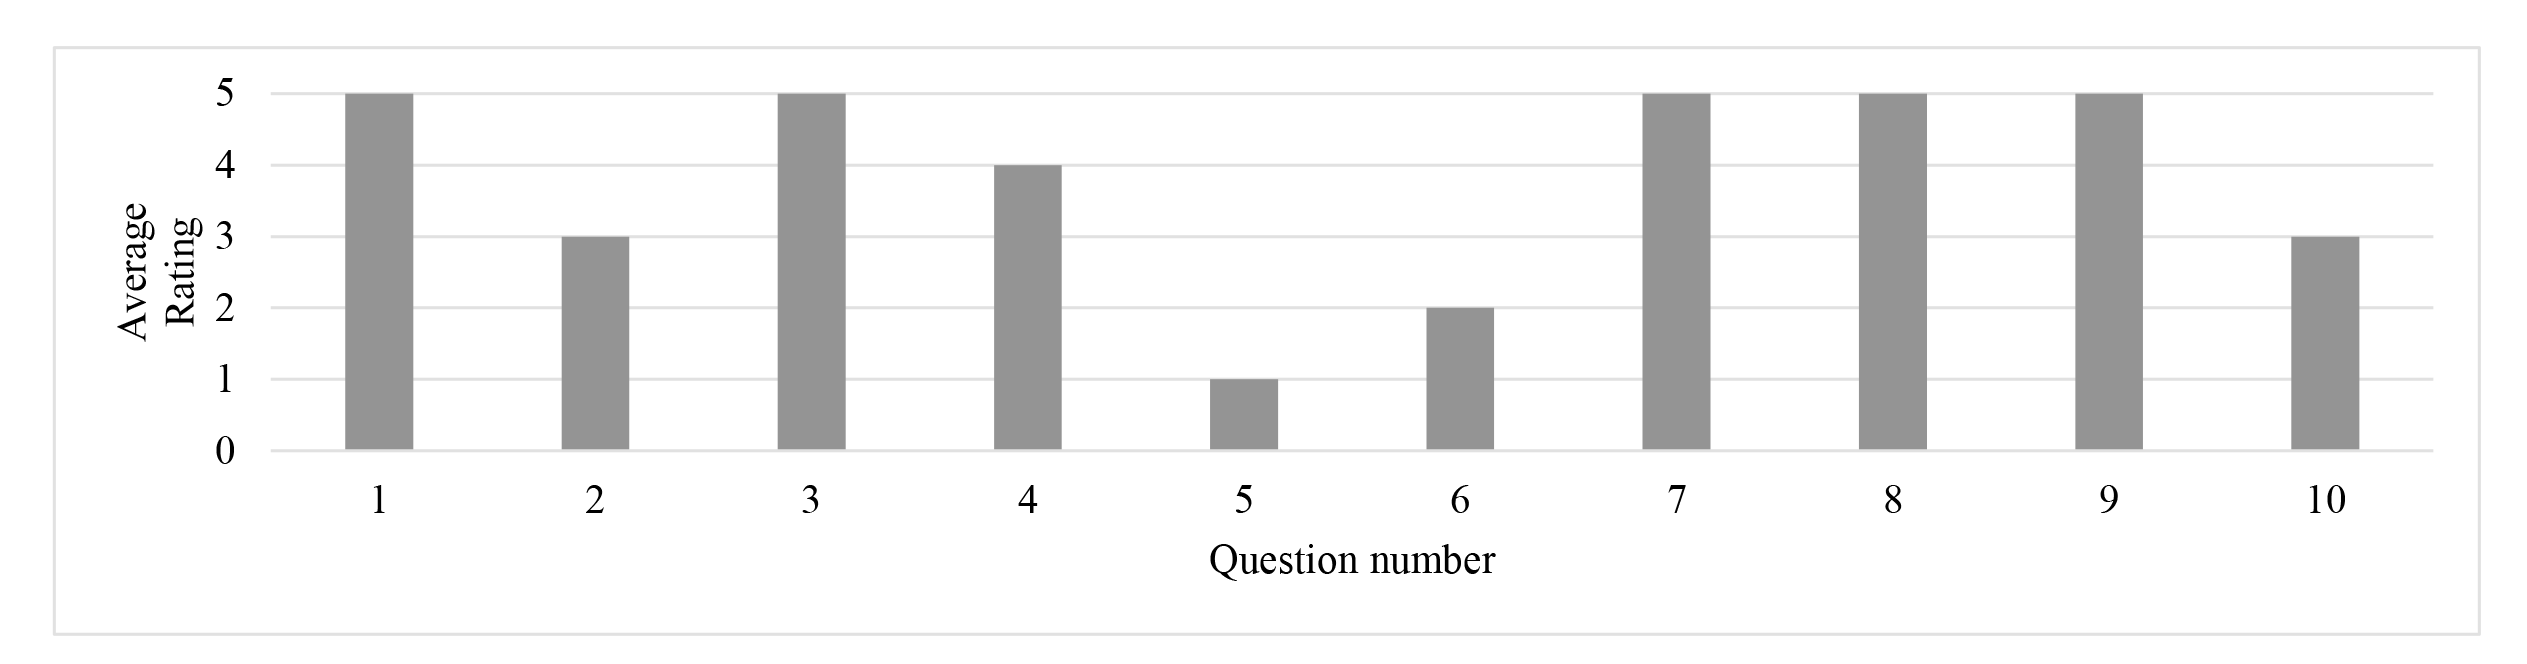
\includegraphics[width=1\textwidth]{figures/task3.png}
    \caption{Task 3 Post-Questionnaire Responses.}
    \label{fig:task3}
\end{figure}

\subsubsection{Discussion}
The usability evaluation proved there were many positive aspects of the Quarters user interface. Every participant was able to complete their task, and in an efficient time, regardless of the browser or the device. The straightforward navigation of the application allowed the participants to navigate easily across the web application and communicate quickly, which is a high-level goal of the software. The questionnaire results showed that participants agreed that Quarters was easy and intuitive to use. Based on these usability results, one could infer that the design and implementation support Norman’s Design Principles, as discussed in the Detailed Design document. The participants of the usability test unanimously strongly agreed that they would use the Maintenance Ticketing, File Upload and Notifications features. After testing Quarters, in response to how frequently they would use Quarters, participants either did not change their mind, or said they would use it more frequently relative to what they had stated prior to testing Quarters. Several participants noted during the ‘talk-aloud’ that they could see Quarters solving a lot of issues they experience in their current households. These positive test results prove that Quarters has marketability. \\ \\
Quarters was not without its weaknesses though. Not every participant saw the value in using Quarters on a daily basis and not every participant would recommend Quarters to a friend. Additionally, Quarters performed poorly on questions 5 and 6, which tested the usability of the Chat feature and the Finances feature, respectively. Participants noted during the ‘talk-aloud’ that they could not see a use for the Chat feature when the Bulletin Board allowed them the same functionality. Additionally, they noted that the purpose of the Finances feature was not initially clear. One landlord noted that they saw value in the File Upload feature, but not so much in the other features. Lastly, some users with a keen eye for design noted some glitches or flaws in our interface. \\ \\
Moving forward, there is room for improvement with regard to the non-functional tests. Removing the Chat feature is something to consider to ensure all of our features collectively integrate well into Quarters. Redesigning the Finances feature or adding more functionality to it may help users understand its purpose more intuitively. Devoting more time and focus to styling would help resolve any design concerns and give the interface a more polished and professional appearance. Hopefully, with these changes, more participants would consider using Quarters more frequently and recommending the application to a friend. The results of the usability test have low external validity; in future usability tests, it would be worthwhile to seek a more diverse testing population outside of a school setting, with more landlords participating. Furthermore, a more complex set of tasks for test participants could give a more accurate reading of the effectiveness and efficiency of our application.
 



\subsection{Performance}
To test the server, we will do a load testing to make sure the server can handle 100 simultaneous requests.

\ds{How?}

\subsection{Robustness}
To test the security of the system, including file access, failed password attempts, SQL injections, and expired sessions, we will do manual testing.

\ds{Be more descriptive.}

\section{Summary of Changes}
\cc{Summarize changes made in response to testing.}


\end{document}
